% MOBISCOPE 프로젝트 보고서 — v0.1 뼈대(skeleton)
% 컴파일: report/README 참조 (xelatex -> bibtex -> xelatex -> xelatex)
% 모든 수치에는 출처를 % 출처: 주석으로 남긴다(docs/report_instructions.md 절대 규칙 3).
% 이 주석은 LaTeX 주석이라 컴파일된 PDF에는 보이지 않는다(눈에 보이는 각주가 아님) — 의도된 동작.
% 주의: 출처 주석은 반드시 "자기만의 줄"에 둘 것 — 문장 끝에 바로 이어 붙이면 그 줄의
% 개행까지 주석이 삼켜서 다음 줄 단어가 띄어쓰기 없이 붙어버린다(v0.1 초안에서 실제로
% 겪은 버그, 이번 수정으로 전부 별도 줄로 옮김).
% docs/notion/의 PDF는 서술 흐름·용어 참고용일 뿐 수치 근거로 쓰지 않았다(우선순위 규칙).

\documentclass[11pt]{article}

\usepackage{kotex}
\setmainhangulfont{Malgun Gothic}

\usepackage[a4paper,margin=2.5cm]{geometry}
\usepackage{graphicx}
\usepackage{booktabs}
\usepackage{tikz}
\usetikzlibrary{arrows.meta,positioning}
\usepackage{float}
\usepackage{authblk}
\usepackage{hyperref}

\renewcommand\Authfont{\normalsize}
\renewcommand\Affilfont{\small\itshape}
\setlength{\affilsep}{1em}

\title{자동차 소프트웨어·전장 결함 조기 탐지를 위한 LLM 기반 조사 Agent:\\
설계, 되감기(backtesting) 평가, 그리고 실험 결과}

\author[1]{주진희\thanks{교신저자(Corresponding author)}}
\author[2]{권효선}
\author[3]{김영운}
\author[4]{윤상진}
\author[5]{허정윤}
\affil[1]{Hankuk University of Foreign Studies \authorcr \texttt{wnwlsgml0112@hufs.ac.kr}}
\affil[2]{Kyungpook National University \authorcr \texttt{kwonhs@knu.ac.kr}}
\affil[3]{Kyung Hee University \authorcr \texttt{k.theodore.yw@khu.ac.kr}}
\affil[4]{Ulsan National Institute of Science and Technology (UNIST) \authorcr \texttt{ysj0708@unist.ac.kr}}
\affil[5]{Hanyang Women's University \authorcr \texttt{huh2815@hywoman.ac.kr}}
\date{2026년 7월}
\begin{document}

\maketitle

\begin{abstract}
본 연구는 NHTSA 소비자 불만 데이터에서 자동차 소프트웨어·전장 결함의 조기 신호를 탐지하는 LLM 기반 조사 Agent를 설계하고, 리콜 발표 이전 시점으로 데이터를 되돌려 평가하는 되감기(backtesting) 프로토콜로 검증했다. 확정한 12개 리콜 사례 중 10건을 포착했으며(평균 선행 215.7일), 신뢰할 수 없는 부품 라벨인 "UNKNOWN OR OTHER" 45건 중 36건을 원본 라벨 앵커링 방식으로 구제했고, 100건 구조화 결과에서 형식 위반과 환각(hallucination)은 각각 0건이었다. 본 보고서는 집중도 가설의 기각을 포함하여, 되감기 기반 평가 프로토콜, 신뢰 불가 라벨 우회 방법론, 가설 기각 사례를 포함하는 실험 결과를 기여로 제시한다.
\end{abstract}

\tableofcontents

\section{서론}

\subsection{문제}

리콜은 결함이 이미 다수 발생한 뒤에야 발표되는 사후적 조치다. NHTSA가 공개하는 소비자 불만 원본은 약 222만 건에 이르는 대규모 비정형 텍스트이며,
% 출처: wc -l data/raw/FLAT_CMPL.txt (2,221,663행)
이를 현대·기아·전장/SW·최근 데이터 기준으로 필터링하면 16,964건이 남는다.
% 출처: data/processed/hk_electrical_recent_full.csv 실측(고유 CMPLID 16,964)
이 중 부품 분류(COMPDESC)가 "UNKNOWN OR OTHER"로 표기된 행이 33.7\%(5,711건)에 달해,
% 출처: data/processed/hk_electrical_recent_full.csv 실측 재계산
부품 라벨 집계만으로는 심각한 결함 신호가 통계에서 누락될 위험이 있다.

소비자 불만 텍스트에서 결함 신호를 찾으려는 시도 자체는 선행 연구에서도 다뤄져 왔다 — NHTSA 불만 데이터에 자연어처리를 적용해 ADAS 결함의 원인-결과 관계를 분석한 연구\cite{ayoub2022adas}나, 소셜미디어 텍스트에서 제품 결함 신호를 추출하는 통합 프레임워크\cite{abrahams2015textanalytic}, 그리고 소비자 불만과 리콜 기록을 결합해 리콜 위험을 예측하는 XGBoost 기반 연구\cite{li2025xgboost}가 그 예다. NHTSA 스스로도 위험 기반 결함 분석·관리 프로세스를 공식 문서로 제시하고 있다\cite{nhtsa2020riskbased}.

\subsection{목표와 설계 원칙}

본 연구의 목표는 이러한 흐름 위에서, 불만 텍스트로부터 리콜보다 먼저 결함 신호를 탐지하는 Agent를 만들고 그 성능을 객관적으로 측정하는 것이다. Agent는 세 가지 설계 원칙을 따른다. 첫째, 폐쇄 근거(closed-context grounding) — 원문에 없는 사실은 생성하지 않는다. 둘째, 불확실성의 명시(모르면 모른다고 말함) — 근거가 부족하면 \texttt{insufficient\_info} 판정으로 보류한다. 셋째, 진단이 아니라는 고지 — 모든 산출물은 미검증 소비자 신고 데이터를 기준으로 함을 명시하고, 결함을 확정하는 표현을 쓰지 않는다.

\subsection{기여}

본 보고서의 기여는 세 가지다.

\begin{enumerate}
\item 되감기(backtesting) 기반의 평가 프로토콜을 구축하였다. 리콜 접수일 이전 데이터만 Agent에 제공한 뒤 실제 리콜 발생 여부로 채점하고, 우연 포착 확률(null model)을 함께 제시하여 절대 포착률만으로 과대평가하지 않도록 하였다.
\item 신뢰할 수 없는 라벨 데이터(COMPDESC)에서 "COMPDESC 앵커링"이라는 우회 방법을 설계하였다. 원본 라벨을 LLM이 재분류하지 않고 관점 지정용 입력으로만 사용하여, 라벨이 부정확한 경우에도 판정의 근거를 원문에서 직접 확인할 수 있도록 하였다.
\item 가설이 기각된 사례를 포함한 실험 결과를 제시하였다. 집중도 가설(5.3)과 같이 예상과 다른 결과가 나온 실험도 결과로서 보고하였다.
\end{enumerate}

\section{배경: 좋은 AI Agent의 조건과 본 주제의 적합성}

\subsection{왜 LLM이 필수인가}

본 프로젝트가 채택한 Agent는 단순 분류기가 아니라, 여러 단계(감지·구조화·조사·판정)를 거치며 각 단계에서 스스로 판단의 근거와 불확실성을 남기는 구조를 갖는다. 이러한 설계가 필요한 이유는 1장에서 확인한 바와 같이 원본 라벨(COMPDESC) 자체가 신뢰할 수 없기 때문이다 — 부품 라벨의 33.7\%가 "UNKNOWN OR OTHER"인 상황에서는 라벨 집계만으로 결함을 판별할 수 없고, 소비자가 직접 작성한 서술문(CDESCR)을 읽고 해석하는 능력이 필요하다. 이것이 규칙 기반 필터링이 아니라 LLM이 필수적인 이유다.

\subsection{LLM과 Agent의 구분}

LLM과 Agent는 구분되는 개념이다. LLM은 주어진 context 안의 정보를 읽고 한 번에 서술을 생성하는 언어 모델이며, 스스로 검색·계산·실행을 수행할 수 없다. Agent는 여기에 도구·기억·판단 루프를 결합해 무엇을 조회할지 스스로 판단하고 그 결과에 따라 다음 행동을 바꾸는 시스템이다. 이 구분에서 LLM의 역할은 사고·판단이고, 실행은 도구에 위임된다.

\subsection{좋은 Agent의 6기준}

이 정의를 기준으로, 좋은 Agent가 갖춰야 할 조건을 여섯 가지로 정리하면 표~\ref{tab:agent-criteria}와 같다.
% 2장의 "LLM vs Agent 구분"과 "좋은 Agent 6기준" 프레임워크 자체는 docs/notion/의
% "I. 들어가며 - 지금까지의 수업 정리와 출발점.pdf" 3~4절(용어·기준 이름)을 그대로 참고했다
% (수치 근거로 쓴 것이 아니라 서술 흐름·용어 참고 — 우선순위 규칙 준수). 대응표의 "본 프로젝트
% 근거" 칸은 전부 code/data 실측 또는 코드 직접 확인(inv02_03_investigation_loop.py 등)만 사용.

\begin{table}[H]
\centering
\small
\begin{tabular}{p{2.1cm}p{3.0cm}p{8.0cm}}
\toprule
기준 & 의미 & 본 프로젝트 근거 \\
\midrule
① 역할 분리 & 계산은 코드, 판단은 LLM &
\texttt{cmplid}·\texttt{odino}·\texttt{compdesc1}·\texttt{compdesc2}는 코드가 원본 COMPDESC를 그대로 파싱해 채우고, \texttt{symptoms}·\texttt{severity}·\texttt{driving\_context}·\texttt{evidence\_quote}·\texttt{insufficient\_info} 5개 필드만 LLM이 판단한다. B1 감지 단계(급증 판정)도 순수 pandas 규칙이라 LLM이 전혀 개입하지 않는다. \\
\addlinespace
② 동적 경로 & 상황에 따라 LLM이 도구·순서를 스스로 선택(고정 파이프라인 아님) &
조사 루프는 가설의 지지 근거가 부족하면 반복마다 조건(연식→모델→키워드 순)을 자동으로 완화해 재조회한다(최대 4회). 다만 이 완화 순서는 LLM이 매번 자유롭게 고르는 것이 아니라 미리 정해둔 순서를 따르는 구조이고, 실제 채팅 진입점에서 사용자 질문에 따라 이 루프를 동적으로 호출하는 연결은 인터페이스 불일치로 아직 끊겨 있다(8장) — \textbf{부분 충족}으로 평가한다. \\
\addlinespace
③ 불확실성 통제 & 증거 부족 시 모름/보류 &
v4 구조화 100건 중 "UNKNOWN OR OTHER" 45건 가운데 9건, 전체로는 14건이 \texttt{insufficient\_info=true}로 보류되었다(5.5절). 조사 루프도 완화된 범위에서 근거 기준에 못 미치면 지지·기각 대신 보류 상태를 반환한다. \\
\addlinespace
④ 자가 검증 & 생성한 답을 스스로 비판·기각하는 루프 &
구조화 단계는 스키마·인용 검증에 실패하면 실패 사유를 프롬프트에 첨부해 최대 3회 재시도한다. 조사 루프는 조건을 다 완화한 뒤에도 근거가 없으면 스스로 가설을 기각한다. Self-Consistency 진단(6장, 안정 68\%/불안정 12\%)으로 판정이 흔들리는 레코드를 식별하는 것도 넓은 의미의 자가검증에 해당한다. \\
\addlinespace
⑤ 추적성 & 모든 주장에 원문 근거(Citation) — 역추적 가능 &
\texttt{evidence\_quote}는 원문(CDESCR)에 실제로 존재하는 연속된 문자열이어야 하며, 100건 검증에서 환각(원문에 없는 인용) 0건을 확인했다(5.5절). 근거가 없는 경우에는 빈 인용 대신 "정보 부족"임을 명시적으로 표시해 있지도 않은 근거를 지어내지 않는다. \\
\addlinespace
⑥ 평가 가능성 & Baseline 대비 개선을 숫자로 증명할 정답지 존재 &
되감기(backtesting) 프로토콜이 리콜 접수일 이전 데이터만 제공한 뒤 실제 리콜 발생 여부를 정답지로 채점한다. K12 12건 중 10건 포착, 우연 포착 확률(0.590)을 함께 제시해 baseline의 개선폭을 수치로 검증했다. \\
\bottomrule
\end{tabular}
\caption{좋은 AI Agent의 6기준과 본 프로젝트의 대응 근거. 기준의 이름과 정의는 수업 자료를 참고했고, 근거 칸은 전부 저장소 code/data 실측이다.}
\label{tab:agent-criteria}
\end{table}

여섯 기준 중 다섯 가지(①③④⑤⑥)는 코드와 실험 결과로 뒷받침되지만, ②동적 경로는 조사 루프 내부의 조건 완화 메커니즘만 실재하고 사용자 질문에 따라 이를 실제로 호출하는 채팅 연결 자체는 끊겨 있어 부분 충족에 그친다.

④ 자가 검증 기준의 검수(Judge) 단계는 강력한 LLM을 사람 평가자의 대리로 사용하는 LLM-as-a-judge 접근과 맞닿아 있다. 이 접근은 GPT-4 수준의 LLM이 사람의 선호와 상당히 일치하는 판단을 내릴 수 있음을 보고한 바 있으며\cite{zheng2023judging}, 4장에서 설계한 교차 벤더 Judge 라우팅도 이와 같은 방향을 따른다. 다만 본 연구에서는 이 라우팅이 코드 수준에서만 확인되었고 실제 판정 실행 결과는 아직 없다(4장, 8장).

\section{데이터}

\subsection{수집 및 필터링}

NHTSA 소비자 불만 원본은 2,221,663행이다.
% 출처: wc -l data/raw/FLAT_CMPL.txt
이를 제조사(현대·기아), 부품 범주(전장/SW 관련 COMPDESC), 접수 시기(2022년 이후) 기준으로 필터링하면 16,964행(고유 CMPLID 16,964, 고유 ODINO 13,974)이 남는다.
% 출처: data/processed/hk_electrical_recent_full.csv 실측
정답지 데이터는 별도로 수집하였다. 미국 리콜은 NHTSA 리콜 API를 통해 현대·기아 차종×캠페인 조합 377행, 고유 캠페인 164개를 확보하였고, 이 중 소프트웨어 관련 후보로 분류된 캠페인은 76개다. 한국 리콜은 국토교통부 보도자료 기반 27건과 한국교통안전공단(KOTSA) 리콜대수 통계 기반 76건을 별도로 수집하였다.
% 출처: data/recalls/recalls_hk_by_vehicle.csv(164개 캠페인), data/recalls/recalls_sw_candidates.csv(76개),
% data/processed/kr_us_gap.csv(27건), data/processed/kr_us_gap_v2.csv(103건=27+76)

\subsection{입력 데이터와 정답지 데이터의 분리}

불만 데이터(입력)와 리콜 데이터(정답지)는 수집 단계부터 별도의 파일 계통으로 관리하였다. 불만 데이터는 Agent가 판단에 사용하는 유일한 근거이고, 리콜 데이터는 그 판단이 실제 결함 대응으로 이어졌는지를 사후에 채점하는 데만 사용한다. 이 분리는 되감기(backtesting) 평가의 전제 조건이다 — Agent에 리콜 정보를 사전에 제공하면 포착 여부를 채점하는 의미가 없어지기 때문이다.

\subsection{되감기 평가 대상(K12) 구축}

소프트웨어 관련 후보 캠페인 76개 중, 접수일 기준 이전 12개월 추이를 확보할 수 있는 캠페인은 46개다(insufficient\_data=False 46건, True 30건).
% 출처: data/processed/lookback_candidates.csv 실측
이 46개 중 12건(K12)을 되감기 평가 대상으로 선정하였다. 선정 기준은 세 가지다. 첫째, 리콜 직전 신고가 급증하는 스파이크형(A, 5건)만으로 구성하면 감지가 쉬운 사례만 고르는 선택 편향이 생기므로, 신고량은 많으나 추이가 평탄한 만성형(B, 4건)과 리콜 5~9개월 전에 먼저 급증했다가 소강하는 조기급증형(C, 3건)을 함께 포함하였다. 둘째, insufficient\_data=True(2022년 이전 리콜)는 제외하였다. 셋째, 한국 리콜과 매칭이 확인된 캠페인(투싼 +8일, 쏘렌토 +10일)을 포함해 한·미 시차 평가와 연동할 수 있도록 하였다.
% 출처: docs/06_되감기_K12_확정.md, docs/k12_list.csv

\subsection{데이터 처리 과정에서 확인된 문제}

원본 데이터의 라벨을 그대로 신뢰할 수 없다는 문제는 본 프로젝트에 한정되지 않는다. 소비자가 직접 카테고리를 선택하는 CFPB 민원 데이터에서도 라벨 오분류(mislabeling) 문제가 지적된 바 있다\cite{bastani_lda_cfpb}. 이는 본 연구가 원본 COMPDESC 라벨을 그대로 신뢰하지 않고 서술문 자체를 읽는 COMPDESC 앵커링 방식을 택한 이유와 맞닿아 있다(4.2절). 데이터 처리 과정에서는 이 밖에도 다음 네 가지 문제를 확인하였다.

\paragraph{필드 수 불일치} FLAT\_CMPL.txt는 NHTSA 공식 스펙 문서상 49개 필드로 정의되어 있으나, 실측 결과 51개 필드가 존재하였다. 나머지 2개(UNKNOWN\_50, UNKNOWN\_51)는 NHTSA가 2021년 이후 추가한 미문서화 컬럼으로, 처리 시점까지 값이 전부 비어 있었다. 스펙 문서 대신 실제 파일의 컬럼 수를 기준으로 파싱하도록 처리하였다.
% 출처: scripts/nhtsa_data_prep.py 컬럼 정의 주석, Import_Instructions_Excel_All.pdf(49개 필드 스펙)

\paragraph{차종명 표기 불일치} B1 신호 발화 목록의 모델명과 미국 리콜 데이터(recalls\_hk\_by\_vehicle.csv)의 모델명 표기가 일치하지 않는 사례가 있었다. 예를 들어 recalls\_hk\_by\_vehicle.csv에는 "TUCSON"만 존재하고 "TUCSON HYBRID"라는 표기는 존재하지 않아, 발화 목록의 "TUCSON HYBRID"는 문자열 단위로 리콜 데이터와 매칭되지 않았다. 이 문제는 집중도 가설 검증(5.3)의 표본을 점검하는 과정에서 발견되었다. HYBRID·PLUG-IN HYBRID·PHEV·ELECTRIC 등 파워트레인 접미어를 제거한 base\_model 기준으로 재정규화한 결과, 정밀도 계산에서 8개 모델-월 조합(SANTA FE HYBRID 2025-08, SONATA HYBRID 2023-10, TUCSON HYBRID 6개월)이 미포착(miss)에서 포착(hit)으로 재분류되었고, 전체 정밀도는 62.7\%(42/67)에서 74.6\%(50/67)로 상향되었다.
% 출처: data/processed/precision_v2.csv 실측 재계산(hit_raw_v1=False, hit_base_observed=True인 행 8건)

\paragraph{한·미 리콜 매칭 오염} KOTSA 리콜대수 통계를 기반으로 한 확장 매칭에서, 시차(gap\_days) 절대값이 365일을 초과하는 사례를 자동으로 "오매칭의심"으로 재분류하는 가드를 적용하였다. 76건 중 13건(17.1\%)이 이 가드에 해당하였으며, 그중 10건은 원래 "한국선행"으로 집계되어 있던 사례였다(상세 결과는 5.4절 참조).
% 출처: data/processed/kr_us_gap_v2_breakdown.csv, scripts/gap_v2_breakdown.py

\paragraph{우측 절단(right-censoring)} 신고 데이터 수집이 2026년 6월에 종료되므로, 발화 시점이 2025년 7월 이후인 신호는 리콜 여부를 채점하는 데 필요한 12개월 관측 기간을 아직 채우지 못한다. B1 발화 67건 중 26건이 이에 해당하였다. 이 26건을 정밀도 계산에서 제외한 결과, 관측 기간이 충족된 41건 중 33건이 리콜로 이어져 정밀도는 80.5\%로 나타났다. 관측 기간이 부족한 26건 중 17건은 이미 부분적인 관측 기간 내에 리콜 연계가 확인되었고, 나머지 9건은 관측 기간이 아직 차지 않아 미포착으로 단정할 수 없는 상태다.
% 출처: data/processed/precision_v2.csv 실측 재계산(censored 컬럼 기준)

\section{시스템 설계}

\subsection{파이프라인 개요}

Agent 파이프라인은 감지(B1) → 구조화(LLM) → 조사 루프 → 판정(Self-Consistency) → 검수(Judge) → 리포트의 6단계로 구성된다. 그림~\ref{fig:pipeline}은 각 단계의 흐름을, 표~\ref{tab:pipeline}은 각 단계의 구현과 관련 기법의 대응을 정리한 것이다.

\begin{figure}[H]
\centering
\begin{tikzpicture}[
  stage/.style={draw, rounded corners, minimum height=1.1cm, minimum width=1.9cm, align=center, font=\small},
  arr/.style={-{Stealth[length=2mm]}}
]
\node[stage] (detect) {감지\\(B1)};
\node[stage, right=0.6cm of detect] (struct) {구조화\\(LLM)};
\node[stage, right=0.6cm of struct] (invest) {조사\\루프};
\node[stage, right=0.6cm of invest] (judge1) {판정\\(Self-\\Consistency)};
\node[stage, right=0.6cm of judge1] (judge2) {검수\\(Judge)};
\node[stage, right=0.6cm of judge2] (report) {리포트};
\draw[arr] (detect) -- (struct);
\draw[arr] (struct) -- (invest);
\draw[arr] (invest) -- (judge1);
\draw[arr] (judge1) -- (judge2);
\draw[arr] (judge2) -- (report);
\end{tikzpicture}
\caption{Agent 파이프라인 6단계.}
\label{fig:pipeline}
\end{figure}

\begin{table}[H]
\centering
\footnotesize
\begin{tabular}{lp{4.3cm}p{3.5cm}p{2.6cm}}
\toprule
단계 & 구현 & 관련 기법 & 비고 \\
\midrule
감지 & \texttt{scripts/b1\_detect.py} (pandas 규칙) & 해당 없음(LLM 미사용) & 검증 완료(5.1절) \\
구조화 & \texttt{scripts/str01\_batch\_structurize.py}\newline\texttt{docs/struct\_prompt\_v4.md} & Structured Output(JSON 스키마 강제)\newline In-Context Learning(few-shot 5개) & 검증 완료(5.5절) \\
조사 루프 & \texttt{scripts/inv02\_03\_investigation\_loop.py} & 반복적 조건 완화 조회 & 채팅 진입점 연결 미완(8장) \\
판정 & \texttt{scripts/str03\_consistency\_analyze\_v4.py} & Self-Consistency(다수결) & 검증 완료(6장) \\
검수 & \texttt{webapp/backend/llm/adapter.py}\newline(MODEL\_MAP) & Verifier Judge(교차 벤더) & 설계 단계, 미실행 \\
리포트 & \texttt{data/processed/report\_24V757000.md} 등 & 근거 인용 포함 서술 생성 & 수동 생성 사례 확인 \\
\bottomrule
\end{tabular}
\caption{파이프라인 단계별 구현과 관련 기법 대응.}
\label{tab:pipeline}
\end{table}
% 출처: 각 셀의 파일 경로는 저장소 실재 파일. Structured Output/ICL: docs/struct_prompt_v4.md
% (responseMimeType=application/json은 scripts/str01_batch_structurize.py의 _call_gemini),
% few-shot 예시 수는 struct_prompt_v4.md의 "예시 1"~"예시 5" 5개 확인.
% 리포트: data/processed/report_24V757000.md, report_false_alarm.md 실재 확인.

\subsection{구조화 단계: COMPDESC 앵커링}

구조화 단계는 원본 COMPDESC 값을 LLM이 재분류하는 대신, 코드가 \texttt{compdesc1}(대분류)/\texttt{compdesc2}(중분류)로 잘라 "이 관점에만 집중하라"는 입력으로 제공한다("COMPDESC 앵커링"). 대분류가 "UNKNOWN OR OTHER"인 경우에 한해서만 같은 신고(ODINO)의 다른 행(형제) COMPDESC를 조회해 "이미 다른 관점에서 처리된 내용은 제외하라"는 근거를 추가로 제공한다(형제 규칙).
% 출처: docs/struct_prompt_v4.md, scripts/str01_batch_structurize.py의 build_sibling_map/sibling_compdescs

\subsection{모델 라우팅}

모델 배정은 단계별로 상이한 모델을 사용하는 구조다. 구조화 단계는 100건·K12 등 반복 실행이 필요한 대량 처리 단계로, Gemini 2.5 Flash(temperature=0)를 사용하였다(5.1~5.5절의 모든 결과가 이 설정으로 산출되었다).
% 출처: data/processed/str01_sample100_v4_fixed_report.md, scripts/str01_batch_structurize.py 실행 로그
웹 서비스(7장)의 조사·응답 단계는 상대적으로 추론 부담이 큰 역할로 분류되어 있어, MODEL\_MAP에서 claude-sonnet-5·gpt-5 등 구조화 단계보다 상위 모델을 배정하도록 설계되어 있다. 검수(judge) 역할은 답변 생성에 사용한 공급사와 항상 다른 공급사로 라우팅되도록 코드에 명시되어 있다(예: Anthropic으로 답변한 경우 OpenAI가 검수). 이 교차 벤더 라우팅은 코드 수준에서 확인되나, 실제 judge 실행 산출물은 존재하지 않는다.
% 출처: webapp/backend/llm/adapter.py의 MODEL_MAP. mock_responses/judge/ 디렉터리는 비어 있음
% (미실행 확인).

\section{실험}

본 장은 각 실험을 가설, 방법, 결과, 판정, 논의의 순서로 서술한다. 가설이 기각된 실험(5.3)의 결과와, 예상과 다른 원인이 확인된 실험(5.4)의 결과를 함께 제시한다.

\subsection{B1 감지 baseline}

\paragraph{가설} 월별 신고 건수에 대한 배율 기반 급증 규칙만으로도, 리콜이 공식 발표되기 전에 결함 신호를 조기에 포착할 수 있다.

\paragraph{방법} 차종(MODELTXT)×월(LDATE) 단위로 신고 건수를 집계해, "당월 건수 $\geq$ 직전 6개월 평균$\times 2$ 그리고 당월 건수 $\geq 10$건"을 만족하면 신호를 발화시키는 규칙을 K12(유형 A 스파이크형 5건, B 만성형 4건, C 조기급증형 3건, 총 12건)에 적용했다. 각 캠페인의 NHTSA 접수일을 컷오프로 그 이전 12개월 창 안에서 발화 여부를 채점했다(대상 차종이 여럿이면 하나라도 발화하면 포착으로 처리). baseline의 "포착"이 순전히 우연이 아닌지 확인하기 위해, 실제 컷오프 대신 2023-07~2026-06 구간 전체를 가상 컷오프로 돌려 "직전 12개월 내 발화가 존재할 확률"(null model)도 별도로 계산했다. 발화가 실제로 결함 대응으로 이어지는지 보기 위한 정밀도는 발화 67건을 대상으로, 차종명 표기(HYBRID 등 파워트레인 접미어) 통일 전후와 관측 기간 충족 여부를 나눠 계산했다.

\paragraph{결과} K12 12건 중 10건을 포착했다(유형 A 4/5, B 3/4, C 3/3), 포착된 10건의 평균 선행일은 215.7일이었다.
% 출처: data/processed/b1_eval_k12.csv
우연 포착 평균 확률은 0.590으로, 실제 포착률(0.833)과 차이가 크지 않았다. 발화 창을 12개월에서 6개월로 좁히면 포착은 10/12에서 8/12로 줄었다.
% 출처: data/processed/b1_eval_validation.csv
정밀도는 원 모델명 기준 62.7\%(42/67)였고, base\_model(파워트레인 접미어 통일) 기준으로는 74.6\%(50/67), 그중 12개월 관측 기간이 충분히 지난 발화만 보면 80.5\%(33/41)였다.
% 출처: data/processed/precision_v2.csv
표~\ref{tab:b1-summary}에 유형별 결과를 정리했다.

\begin{table}[H]
\centering
\small
\begin{tabular}{lccc}
\toprule
유형 & 포착/전체 & 우연 포착 평균 확률 & 비고 \\
\midrule
A(스파이크형) & 4/5 & 0.594 & 5건 평균(0.361, 0.833, 0.833, 0.611, 0.333) \\
B(만성형) & 3/4 & 0.646 & 25V649000·24V879000 두 건 놓침(아래 참조) \\
C(조기급증형) & 3/3 & 0.509 & 3건 평균(0.333, 0.833, 0.361) \\
\midrule
전체 & 10/12 & 0.590 & 실제 포착률 0.833과 대조 \\
\bottomrule
\end{tabular}
\caption{K12 유형별 B1 감지 결과. 우연 포착 평균 확률은 data/processed/b1\_eval\_validation.csv의 chance\_capture 값을 유형별로 평균한 것이다.}
\label{tab:b1-summary}
\end{table}

놓친 2건은 둘 다 유형 B(만성형)였고, 원인은 배율 조건 자체의 구조적 한계였다. SORENTO(25V649000, 컷오프 2025-09-25)는 컷오프 전 12개월 월별 건수가 14~30건 사이였으나, 직전 6개월 평균(baseline)도 이미 20.3~37.7건대로 함께 높아 배율(2배) 조건을 넘지 못했다. ELANTRA·SANTA FE(24V879000, 컷오프 2024-11-21)도 마찬가지로 월별 건수(ELANTRA 9~43건, SANTA FE 10~27건)와 baseline(각각 18.3~30.2건대, 16.0~21.0건대)이 나란히 높은 수준에서 움직여 스파이크로 잡히지 않았다.
% 출처: data/processed/b1_signals.csv 실측 재계산(SORENTO·ELANTRA·SANTA FE 해당 구간)

\paragraph{판정} 표면적인 포착률(10/12=83.3\%)만 보면 양호해 보이지만, 우연 포착 확률(0.590)과의 격차가 크지 않고 정밀도도 최대 80.5\%에 그쳐(발화 5건 중 1건은 12개월 내 리콜로 이어지지 않음) "감지만으로는 결함을 규명할 수 없다"고 판정한다.

\paragraph{논의} 배율 기반 규칙은 절대 건수 자체가 이미 만성적으로 높은 상태에서 완만히 유지되는 유형(유형 B)을 구조적으로 놓친다. 감지 단계가 할 수 있는 일은 "주목할 후보를 좁히는 것"까지이며, 그 후보가 실제로 결함을 가리키는지는 서술문을 읽어야 알 수 있다 — 이것이 LLM 기반 구조화·조사 단계가 필요한 근거다.

\subsection{구조화 판정 규칙 보정}

\paragraph{가설} 초기 구조화 프롬프트(v1, 심각도 판정 기준이 "주행 안전 직결성" 단일 원칙)는 사고·부상 이력이나 통제 가능한 편의 기능 고장까지 CRITICAL로 과대평가할 수 있다.

\paragraph{방법} 20건 미니테스트(v1) 결과를 검토한 뒤, ISO 26262의 Controllability(통제가능성) 개념 등을 반영한 판정 규칙 3종 — ① 결함-결과 분리(사고·부상이 결함과 인과관계로 명시되지 않으면 severity에 반영하지 않음), ② 통제 가능성(후방카메라·인포테인먼트 등 대체 가능한 기능은 SERIOUS 상한, 제동·조향·동력 등 대체 불가 기능만 CRITICAL 허용), ③ 오작동$>$미작동(안전장치의 자의적 개입은 미작동보다 한 단계 높게 판정) — 을 프롬프트에 명시적으로 추가해 v2를 만들었다. v1의 20건 각각에 대해 v2 규칙 적용 시 재판정이 바뀌는지 대조했다.
% 출처: docs/struct_prompt_v2.md

\paragraph{결과} 20건 중 2건이 규칙 적용 후 재판정이 바뀌었다. 나머지 18건은 v1과 v2의 판정(part\_category·severity·driving\_context·insufficient\_info·symptoms)이 전부 동일했다(무변화 18/18).
% 출처: data/processed/llm_struct_test_v2_regression.csv

\begin{table}[H]
\centering
\small
\begin{tabular}{lp{5.5cm}cc}
\toprule
ODINO & 증상 & v1 severity & v2 severity \\
\midrule
11551510 & 후방카메라 화면 오류, 블라인드스팟 센서 오작동 & CRITICAL & SERIOUS \\
11729316 & 차선이탈 경고 미작동, 차선이탈 후 중앙분리대 충격 & CRITICAL & SERIOUS \\
\bottomrule
\end{tabular}
\caption{v2 규칙 적용으로 재판정이 바뀐 경계 사례 2건. 둘 다 규칙②(통제 가능성 — 후방카메라·경고성 ADAS는 대체 가능한 기능이라 SERIOUS 상한)가 적용됐다.}
\label{tab:v1v2-boundary}
\end{table}
% 출처: data/processed/llm_struct_test_results.jsonl(v1 값), 커밋 492fffb 메시지(v2 재판정 기록),
% docs/struct_prompt_v2.md 규칙②

\paragraph{판정} 20건 중 2건(10\%)에서 실제로 과대평가가 확인되었고, 두 사례 모두 규칙②로 설명되는 동일한 패턴(대체 가능한 편의·경고 기능의 고장을 CRITICAL로 판정)이었다. 나머지 18건(90\%)은 v1이 이미 새 규칙과 암묵적으로 일치하는 판단을 하고 있었다 — v1이 전반적으로 크게 어긋나 있었던 것은 아니지만, 규칙을 명시하지 않으면 경계 사례에서 재현 가능하지 않은 방식으로 흔들릴 수 있음을 확인했다.

\paragraph{논의} 결과만 보면 괜찮아 보이는 프롬프트라도 "왜 그렇게 판단했는지"가 규칙으로 명문화돼 있지 않으면 경계 사례의 일관성을 보장할 수 없다. 규칙을 추가한 뒤 회귀 검증으로 "그 규칙이 기존 판단을 실제로 얼마나 바꾸는지"를 직접 측정하는 편이, 프롬프트를 바꾸고 그대로 믿는 것보다 안전하다.

\subsection{집중도 가설 검증}

\paragraph{가설} B1 발화 시점의 part\_category 최빈 비율(집중도)이 높을수록, 그 발화가 실제 리콜로 이어질 가능성이 높다.

\paragraph{방법} 먼저 소규모 대조(n=2)로 방향성을 확인했다: EV9(2024-09, 실제 24V757000 리콜로 이어짐)의 집중도는 0.966(INSTRUMENT\_CLUSTER)이었고, GENESIS(2024-04, 12개월 내 리콜로 이어지지 않음)의 집중도는 0.571(ELECTRICAL\_SYSTEM)이었다 — 리콜로 이어진 쪽이 훨씬 높아 가설이 유망해 보였다. 이를 검증하기 위해 B1 발화 67건을 리콜연계(12개월 내 리콜)/비연계 그룹으로 나눠 각 5건씩 총 10건을 무작위 추출했다(seed=42, EV9·GENESIS 강제 포함).
% 출처: data/processed/concentration_test.csv, CLAUDE.md Task 8

\paragraph{결과} 표본 10건에서 리콜연계 그룹의 평균 집중도는 0.645(중앙값 0.733), 비리콜 그룹은 0.661(중앙값 0.571)로, 비리콜 그룹이 오히려 근소하게 더 높았다.
% 출처: data/processed/concentration_test.csv 실측 재계산
표~\ref{tab:concentration}에 10건 전체를 정리했다. 표본 최고 집중도(CARNIVAL, 2024-08, 1.000 — 기생 배터리 방전 단일 원인)는 비리콜 그룹이었고, 표본 최저 집중도 2건(PALISADE 0.300, KONA 0.357)은 둘 다 실제 리콜로 이어진 사례였다 — 가설과 정반대 방향의 극단 사례였다. 이후 차종명 표기를 통일(HYBRID 접미어 정규화)해 표본을 재분류한 결과에서도(리콜연계 n=7, 평균 0.637·중앙값 0.700 / 비리콜 n=3, 평균 0.690·중앙값 0.571) 비리콜 그룹 평균이 여전히 근소하게 높았다.
% 출처: data/processed/concentration_test_v2.csv

\begin{table}[H]
\centering
\small
\begin{tabular}{llcc}
\toprule
차종·월 & 그룹 & 최빈 part\_category & 집중도 \\
\midrule
CARNIVAL 2024-08 & 비리콜 & PROPULSION\_BATTERY & 1.000 \\
EV9 2024-09 & 리콜연계 & INSTRUMENT\_CLUSTER & 0.966 \\
IONIQ 5 2025-03 & 리콜연계 & PROPULSION\_BATTERY & 0.867 \\
IONIQ 5 2023-05 & 리콜연계 & PROPULSION\_BATTERY & 0.733 \\
TUCSON HYBRID 2025-05 & 비리콜 & ADAS & 0.700 \\
GENESIS 2024-04 & 비리콜 & ELECTRICAL\_SYSTEM & 0.571 \\
TUCSON HYBRID 2025-07 & 비리콜 & INSTRUMENT\_CLUSTER & 0.533 \\
K4 2026-02 & 비리콜 & ADAS & 0.500 \\
KONA 2025-08 & 리콜연계 & ELECTRICAL\_SYSTEM & 0.357 \\
PALISADE 2022-08 & 리콜연계 & POWERTRAIN\_SW & 0.300 \\
\bottomrule
\end{tabular}
\caption{집중도 가설 검증 표본 10건. 리콜연계 평균 0.645(중앙값 0.733), 비리콜 평균 0.661(중앙값 0.571).}
\label{tab:concentration}
\end{table}

\paragraph{판정} n=2에서 유망해 보였던 방향성은 n=10에서 뒤집혔고, 차종명 재분류 후에도 결론은 바뀌지 않았다 — "집중도 단일 지표"가 리콜 연계 여부를 가르는 신뢰할 수 있는 기준이라는 가설은 기각한다.

\paragraph{논의} 표본 2건의 관찰은 우연히 방향이 맞아떨어졌을 뿐이었다. part\_category 집중도는 결함의 "성격"(단일 원인인지 복합 원인인지)을 반영할 뿐, 그 결함이 "심각한지" 또는 "리콜로 이어질지"와는 별개다 — 리콜 판정은 단일 지표가 아니라 다기준으로 접근해야 함을 재확인했다.

\subsection{한·미 매칭 검증}

\paragraph{가설(관측)} KOTSA 리콜대수 통계를 기반으로 미국·한국 리콜을 확장 매칭한 결과(76건), 한국이 미국보다 먼저 리콜을 시작한 사례(한국선행)가 38건으로 미국선행(31건)보다 많아, "한국이 리콜 대응에서 더 빠르다"는 관측이 나왔다.
% 출처: data/processed/kr_us_gap_v2.csv(date_basis=KOTSA리콜개시일, 76행) 실측 재계산

\paragraph{방법} 이 방향성 통계를 그대로 신뢰하기 전에, 시차(gap\_days) 절대값이 365일을 초과하는 사례를 "오매칭의심"으로 재분류하는 가드를 적용해 매칭 신뢰도를 점검했다.
% 출처: scripts/gap_v2_breakdown.py

\paragraph{결과} 76건 중 13건(17.1\%)이 이 가드에 걸려 오매칭의심으로 재분류되었다. 이 13건 중 10건이 원래 "한국선행"으로 집계돼 있던 사례였다(시차 최대 $-$635일). 가드 적용 후 분류는 한국선행 28건, 미국선행 28건으로 정확히 같아졌다.
% 출처: data/processed/kr_us_gap_v2_breakdown.csv 실측 재계산
반면 국토부 보도자료 기반의 소규모 매칭(27건, kr\_us\_gap.csv)에서는 투싼(26V400000, +8일)처럼 개별적으로 확인된 사례가 남아 있다.

\paragraph{판정} KOTSA 기반 확장 매칭(76건)에서 관측된 "한국선행이 더 많다"는 방향성 통계는 신뢰할 수 없다고 판정한다. 애초 우위로 보였던 "한국선행 38건"의 약 4분의 1(10건)이 시차가 최대 635일에 달하는 오매칭 의심 사례였기 때문이다. 개별 검증이 끝난 소수(보도자료 기반 27건)만 신뢰하는 방향으로 결론을 후퇴시킨다.

\paragraph{논의} 자동 매칭 파이프라인에서 산출된 방향성 통계(어느 쪽이 몇 건 더 빠른가)는 매칭 오류에 특히 취약하다. 표본 수를 늘리는 것보다 이상치를 걸러내는 가드와 개별 사례 검증이 선행되어야 한다.

\subsection{v4 구조화 전환 및 100건 검증}

\paragraph{가설} 원본 COMPDESC 값을 LLM이 다시 분류하게 하는 대신, 코드가 그대로 파싱해 "이 관점에만 집중하라"는 입력으로 제공하면(COMPDESC 앵커링), 라벨이 부정확할 수 있는 "UNKNOWN OR OTHER" 사례에서도 형식 위반이나 환각 없이 유의미한 판정을 끌어낼 수 있다.

\paragraph{방법} hk\_electrical\_recent\_full.csv(16,964행)에서 100건을 표본 추출했다 — 다중 CMPLID 앵커링 검증용(A, 27행), UNKNOWN+형제 있음(B, 13행), UNKNOWN+형제 없음(C, 13행), 무작위(RANDOM, 47행) 4개 그룹으로 구성했다. docs/struct\_prompt\_v4.md·Gemini 2.5 Flash·temperature=0으로 CMPLID 단위 구조화를 실행했고, COMPDESC 대분류가 "UNKNOWN OR OTHER"인 경우에만 같은 신고(ODINO)의 다른 행(형제) COMPDESC를 원본 전체에서 조회해 "이미 처리된 내용은 배제하라"는 근거로 추가 제공했다. 결과는 스키마 검증(필수 9필드·허용값)과 인용 검증(evidence\_quote가 원문에 실제로 존재하는지)으로 독립 재검사했다.
% 출처: scripts/sample_v4_100.py, docs/struct_prompt_v4.md, scripts/str01_batch_structurize.py

\paragraph{결과} 100/100건 완주, 형식 위반 0건, 환각(원문에 없는 인용) 0건이었다(insufficient\_info=true 14건은 빈 인용 예외로 별도 허용).
% 출처: data/processed/str01_sample100_v4_fixed_report.md
"UNKNOWN OR OTHER" 45건 중 11건은 형제 COMPDESC를 조회해 그 내용을 제외한 나머지로 구체적인 판정을 끌어냈고, 25건은 형제가 없어 서술문 전체에서 가장 두드러진 결함으로 판정했다(둘을 더해 36/45=80.0\%가 정보 부족 없이 처리됨). 나머지 9건은 형제 내용을 제외하고 나니 판단할 근거가 남지 않아 \texttt{insufficient\_info=true}로 표시되었다(전체 100건 기준 insufficient 14건).
% 출처: 본 세션 재검증(scripts/str01_batch_structurize.py의 build_sibling_map/sibling_compdescs 재사용)
severity 분포는 CRITICAL 61 / SERIOUS 23 / MINOR 9 / MODERATE 7이었다.
% 출처: data/processed/str01_sample100_v4_fixed_report.md

\begin{table}[H]
\centering
\small
\begin{tabular}{lc}
\toprule
UNKNOWN OR OTHER 45건 처리 결과 & 건수 \\
\midrule
형제 COMPDESC 조회로 구제 & 11 \\
형제 없이 본문 전체로 판단 & 25 \\
insufficient\_info=true로 보류 & 9 \\
\bottomrule
\end{tabular}
\caption{UNKNOWN OR OTHER 45건의 v4 처리 결과 분해.}
\label{tab:v4-unknown}
\end{table}

\paragraph{판정} 원본 라벨을 재분류하지 않고 앵커로만 쓰는 설계는, "라벨이 부정확할 수 있으므로 배제하지 않는다"는 이 프로젝트의 원칙과 "환각 없이 유의미한 판정을 끌어낸다"는 목표를 동시에 만족시켰다고 판정한다.

\paragraph{논의} 라벨 자체를 못 믿을 때 LLM에게 "라벨을 대신 정하라"고 요청하는 대신 "기존 라벨을 관점으로 삼아 그 관점에서만 원문을 읽어라"고 요청하는 것이 더 안전한 우회로였다. UNKNOWN OR OTHER처럼 구조적으로 정보가 적은 라벨에서도, 같은 신고의 다른 행(형제)이라는 문서 내부 구조를 활용하면 정보 부족 비율을 줄일 수 있었다.

\section{평가 방법론}

\subsection{되감기(backtesting) 프로토콜}

되감기 프로토콜은 리콜 접수일 이전 데이터만 Agent에 제공한 뒤, 포착 여부·선행 일수·근거 정확성을 채점하는 방식이다. NHTSA가 공식적으로 채택하고 있는 위험 기반 결함 관리 절차\cite{nhtsa2020riskbased}와 마찬가지로, 본 프로토콜도 결함 대응 여부를 사후적으로가 아니라 시점을 되돌려 평가한다는 점에서 조기 경보 성격의 평가 설계에 해당한다. 우연히 포착될 확률(null model)을 병기하여 절대 포착률만으로 과대평가하지 않도록 하였다(5.1절).

Self-Consistency 진단(동일 100건을 temperature=0.4로 3회 반복)에서는 판정이 안정적으로 유지된 레코드가 68\%, 부분적으로 흔들린 레코드가 20\%, 완전히 갈린 레코드가 12\%였다.
% 출처: data/processed/str03_consistency_v4_fixed_report.md

\subsection{골드라벨 교차 채점}

골드라벨 교차 채점(5인 독립 채점 후 다수결로 정답을 확정하는 방식)과 이를 통한 Judge 신뢰도 검증은 방법이 설계되어 있으나 채점은 아직 시작되지 않았다 — 채점 시트(\texttt{data/samples/grading\_sheet*.csv})는 채점 대상(severity·symptoms·insufficient\_info, 부품은 원본 라벨이므로 제외)이 정의된 상태로 존재하나, 채점 항목은 현재 전부 공란이다.
% 출처: data/samples/grading_sheet.csv, grading_sheet_v2.csv, grading_sheet_v4.csv 실측(채점 컬럼 전부 결측)
채점이 완료되면 채점자 간 일치도(Inter-Annotator Agreement, IAA)를 산출할 계획이다. IAA 산출 방법론은 전산언어학 분야에서 정립되어 있으며\cite{artstein2008intercoder}, 강력한 LLM을 채점자로 쓰는 LLM-as-a-judge 접근이 사람 선호와 상당한 일치를 보인다는 보고\cite{zheng2023judging}를 참고해, 향후 교차 벤더 Judge 설계(4장)의 신뢰도를 이 IAA 값으로 검증할 예정이다.

\subsection{이층 평가 체계}

본 연구의 평가는 두 층위로 구성된다. 모듈 평가는 구조화 단계 하나만을 사람이 직접 채점하는 방식으로, 골드라벨 교차 채점이 여기에 해당한다. 시스템 평가는 감지부터 판정까지 파이프라인 전체를 되감기 프로토콜로 채점하는 방식으로, 5장의 K12 실험이 여기에 해당한다. 모듈 평가는 세부 판정(예: severity가 맞았는지)을 검증하고, 시스템 평가는 결과적으로 리콜을 더 일찍 포착했는지를 검증한다는 점에서 서로 다른 질문에 답한다.

\section{웹 서비스 구현}

\subsection{화면 구성}

웹 서비스는 상황판(대시보드)·조사 채팅·내 차(3D) 3개 화면으로 구성된다. 상황판은 KPI 요약, 한·미 시차 덤벨 차트, 신고 히트맵을 보여준다(그림~\ref{fig:dashboard}). 조사 채팅은 질문을 입력하면 단계별 조사 과정을 스트리밍으로 보여준 뒤 원문 인용을 포함한 답변을 제시한다(그림~\ref{fig:chat}). 내 차 화면은 등록한 차종의 3D 모델 위에 도메인별(전장·ADAS 등) 상태를 핫스팟으로 표시한다(그림~\ref{fig:mycar}).
% 출처: docs/screenshots/{dashboard,chat,mycar}.png (2026-07-08 Playwright 촬영). 이후 UI가
% 여러 차례 개편되어(CLAUDE.md 7.6~7.17단계) 현재 화면과 세부 배치가 다를 수 있다.

\begin{figure}[H]
\centering
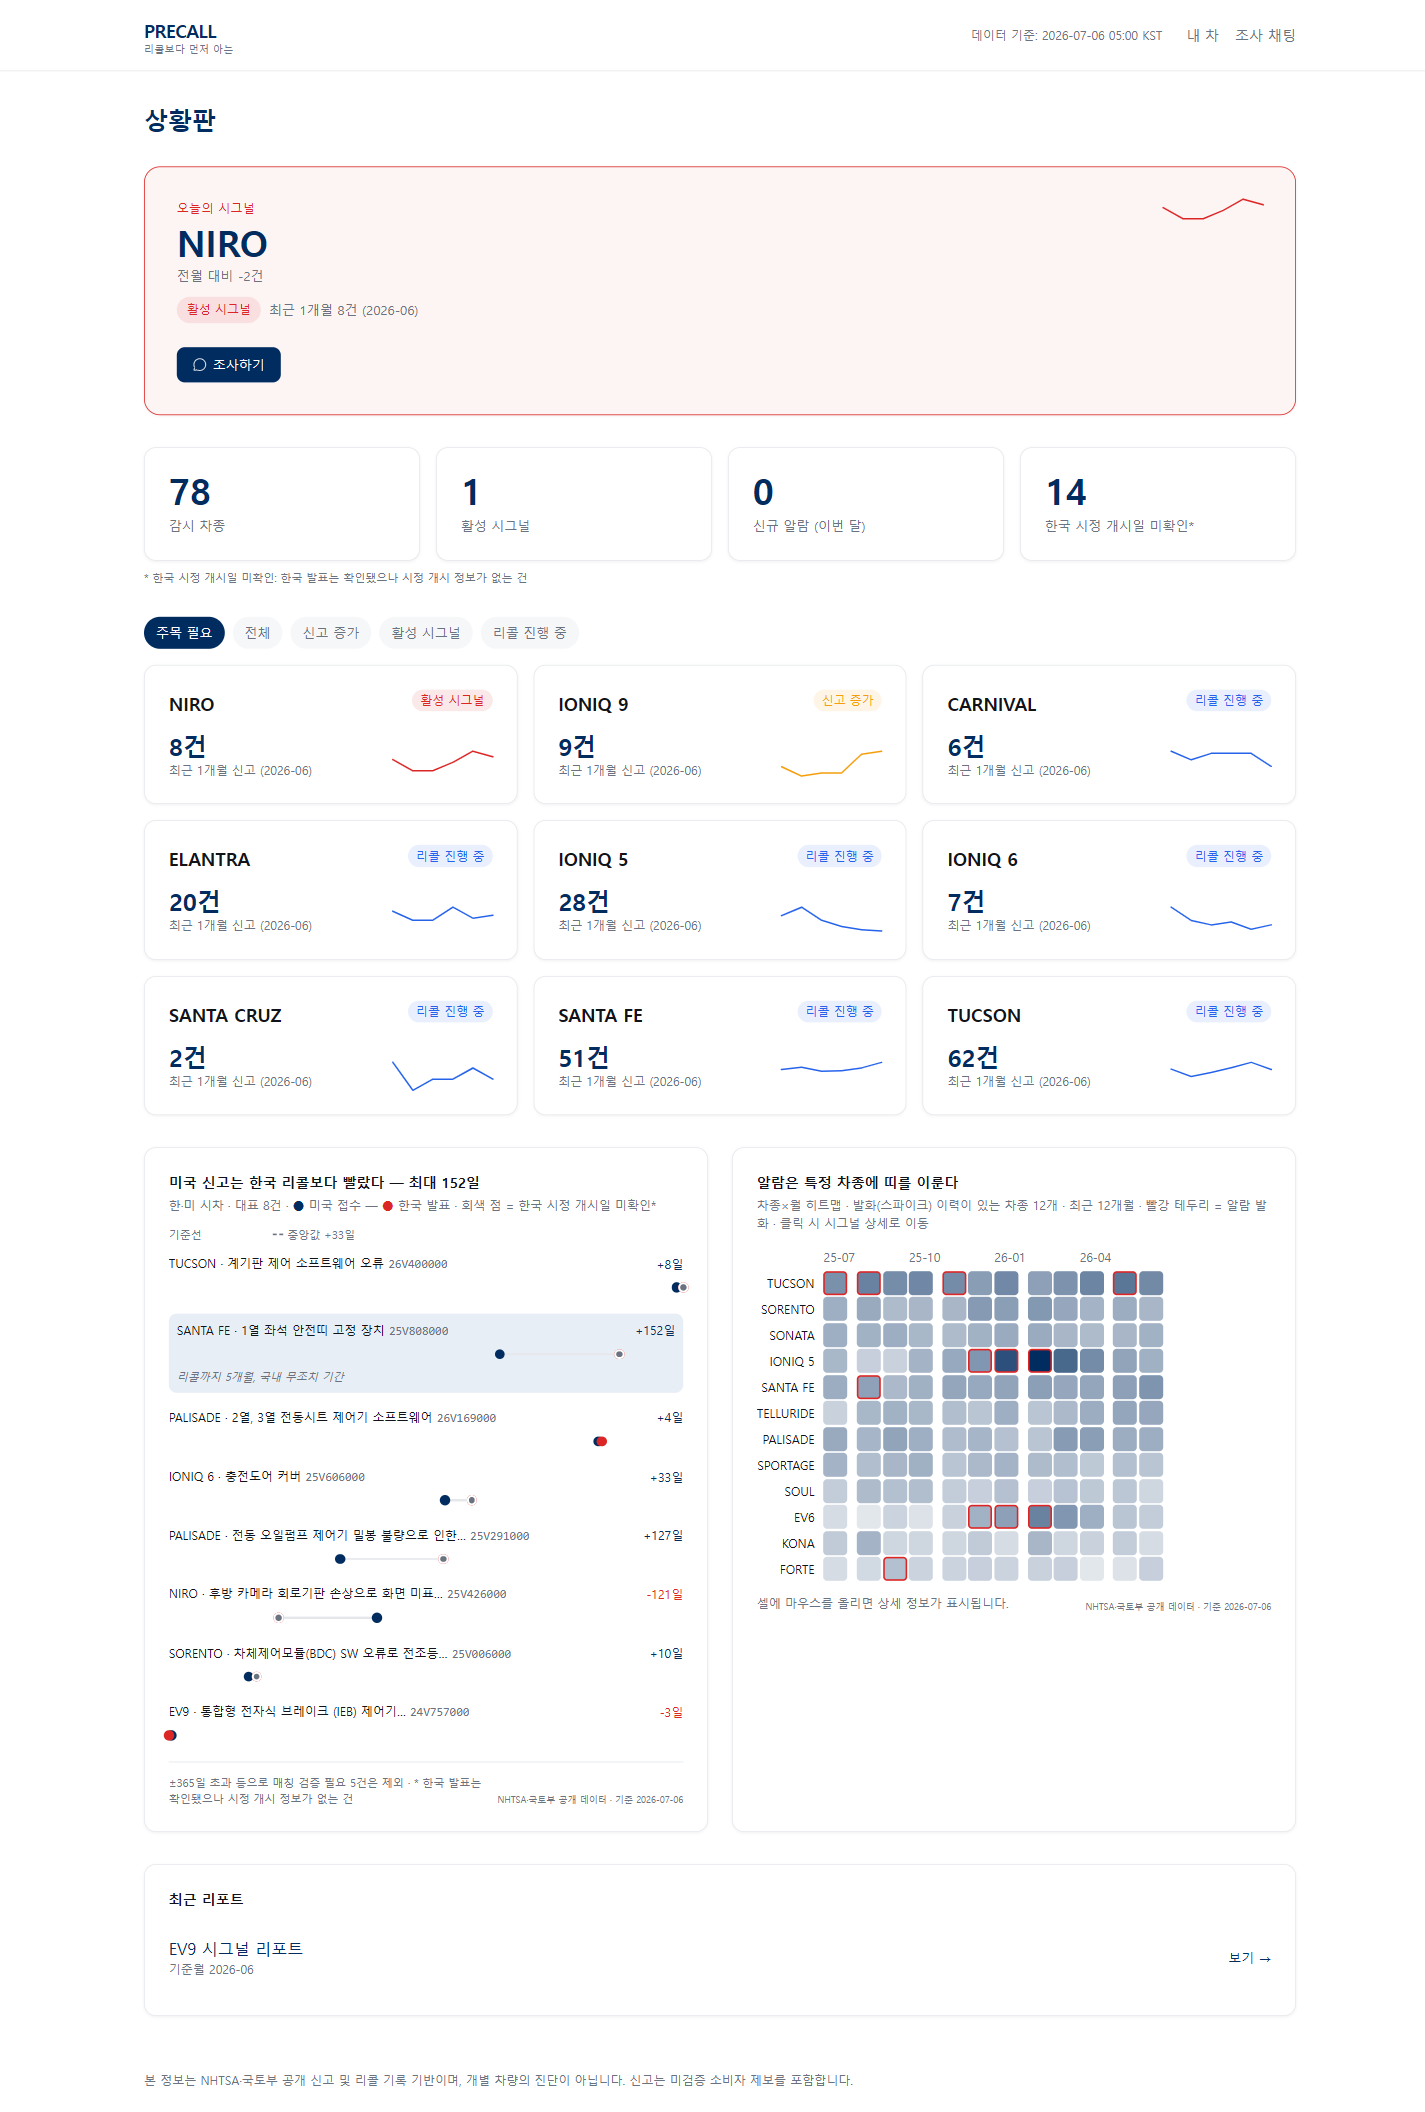
\includegraphics[width=0.8\textwidth]{../docs/screenshots/dashboard.png}
\caption{상황판(Dashboard) 화면. KPI 요약, 한·미 시차 덤벨 차트, 신고 히트맵을 보여준다.}
\label{fig:dashboard}
\end{figure}

\begin{figure}[H]
\centering
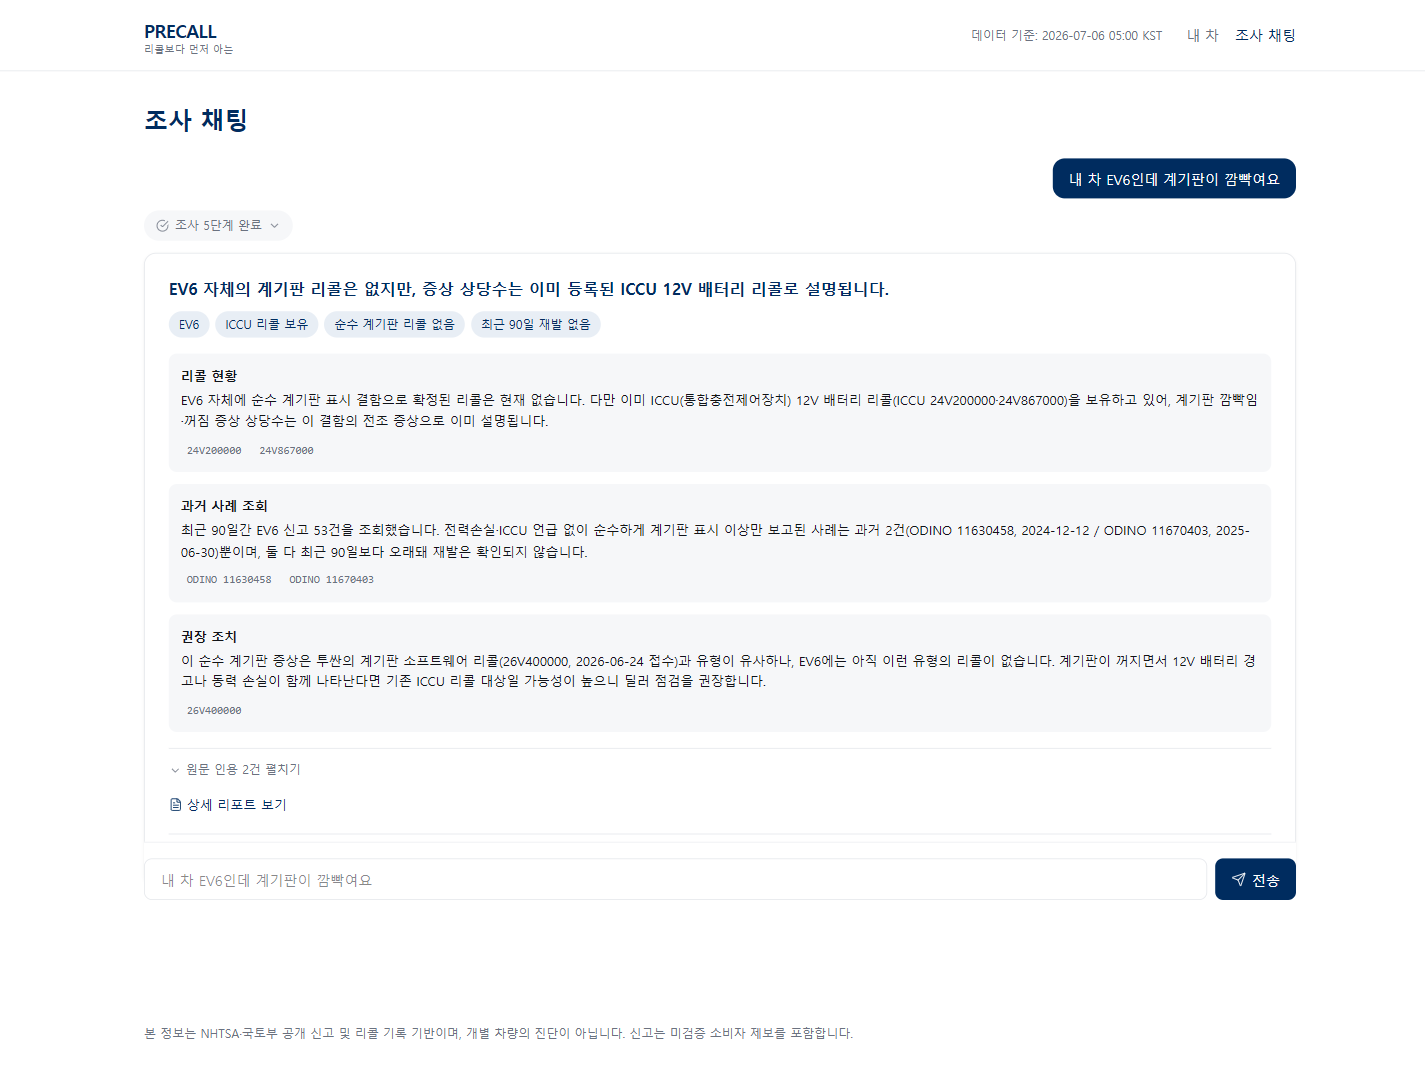
\includegraphics[width=0.8\textwidth]{../docs/screenshots/chat.png}
\caption{조사 채팅 화면. 질문 입력 후 단계별 조사 과정과 원문 인용을 포함한 답변을 보여준다.}
\label{fig:chat}
\end{figure}

\begin{figure}[H]
\centering
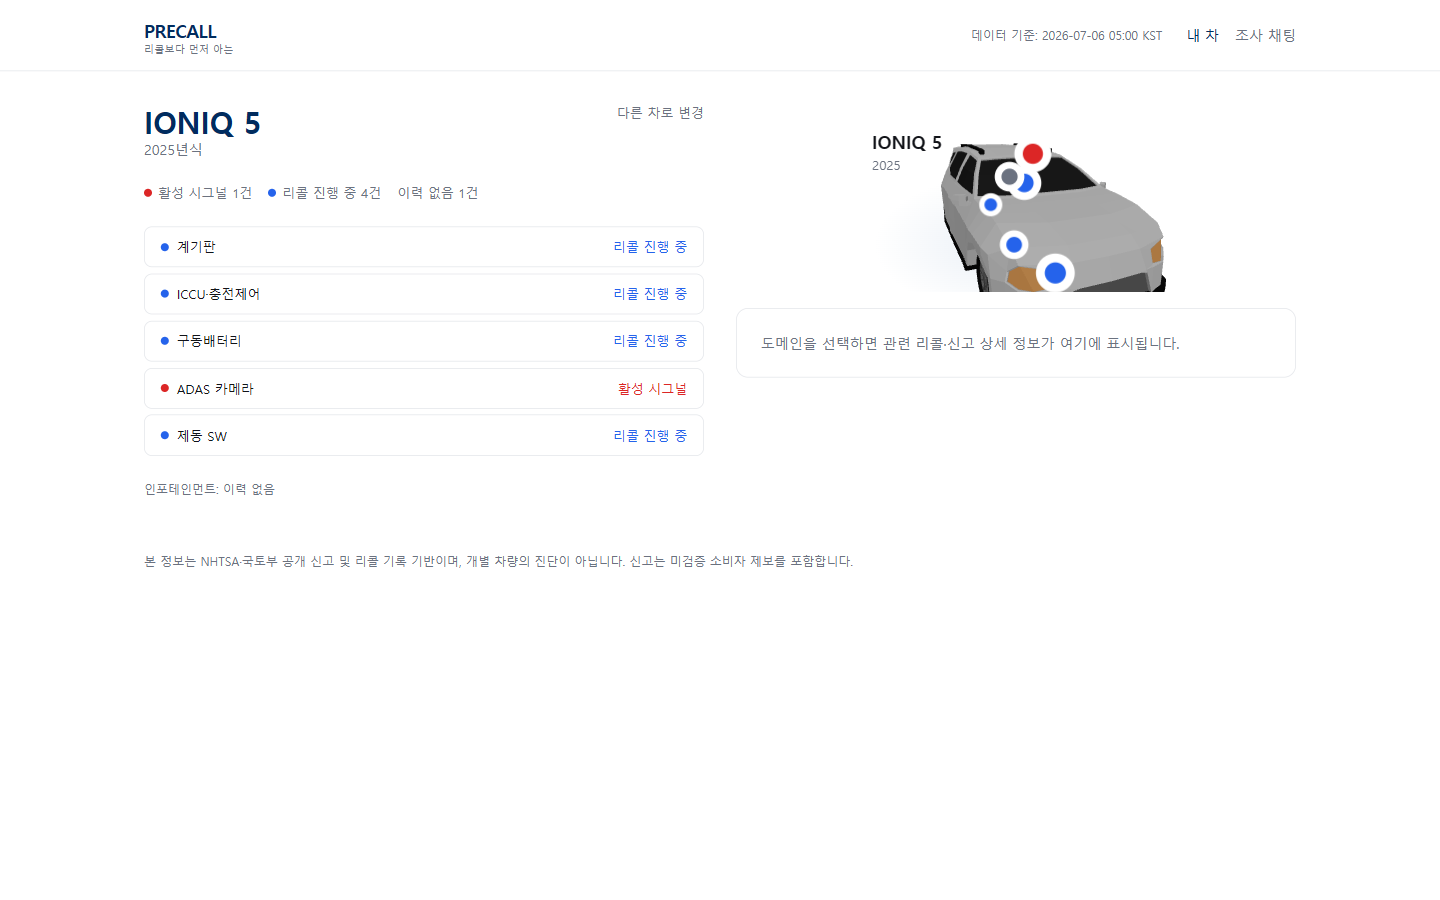
\includegraphics[width=0.8\textwidth]{../docs/screenshots/mycar.png}
\caption{내 차 화면. 등록 차종의 3D 모델 위에 도메인별 상태를 핫스팟으로 표시한다.}
\label{fig:mycar}
\end{figure}

\subsection{조사 채팅 데모 시나리오}

조사 채팅은 키워드 매칭으로 3개 시나리오(ev6\_cluster·ioniq5\_charging·out\_of\_scope) 중 하나로 분기한 뒤, Server-Sent Events(SSE)로 조사 단계를 순차 스트리밍한다. 각 단계에서 표시되는 수치(신고 건수·리콜 캠페인 번호 등)는 템플릿에 미리 적어둔 값이 아니라, 매 요청마다 데이터베이스에서 직접 조회하여 채워 넣는다.
% 출처: webapp/backend/routers/chat.py, webapp/backend/llm/adapter.py
ev6\_cluster 시나리오는 EV6 차종의 계기판 관련 신고를 조사하는 과정을 보여준다. 이 시나리오를 구성하는 과정에서, EV6가 이미 ICCU(통합충전제어장치) 12V 배터리 관련 리콜(24V200000, 이후 24V867000으로 확대)의 대상 차종이며, "계기판이 깜빡이다 꺼짐" 유형 신고 대부분이 이 기존 리콜로 설명된다는 사실을 확인하였다. 데모 시나리오는 이 사실을 반영하여, 최근 90일 신고 중 순수 계기판 표시 결함만 보고된 사례가 이미 이 기존 리콜과 무관한 것으로 확인된 결과를 보여주도록 구성되어 있다.
% 출처: data/recalls/recalls_hk_by_vehicle.csv(EV6 리콜 이력), webapp/backend/llm/mock_responses/answer/ev6_cluster.json

\subsection{목 모드 어댑터}

LLM API 키가 설정되지 않은 환경에서도 데모가 동작하도록, 어댑터는 \texttt{LLM\_PROVIDER} 환경변수가 없으면 자동으로 목(mock) 모드로 전환된다. 목 모드는 \texttt{llm/mock\_responses/\{role\}/\{scenario\}.json}의 템플릿에 실시간 조회 결과를 대입하여 반환하므로, 응답에 포함되는 수치는 실제 데이터베이스 조회값이다.
% 출처: webapp/backend/llm/adapter.py

\section{한계와 향후 과제}

\subsection{한계}

일부 모듈은 아직 통합되지 않았다. 채팅 파이프라인(\texttt{cht01\_chat\_pipeline.py})이 기대하는 조사 모듈 인터페이스(함수 시그니처·모듈명)와 실제로 구현된 조사 모듈(\texttt{inv01\_query\_templates.py}, \texttt{inv02\_03\_investigation\_loop.py})이 서로 달라, 이 연결은 실행되지 않는 상태로 남아 있다.
% 출처: scripts/cht01_chat_pipeline.py의 import 대상과 실제 파일명·함수 시그니처 대조(diff 확인)
B1 감지의 정밀도(5.1절, 최대 80.5\%)는 NHTSA 정식 리콜만을 "결함 대응"의 기준으로 삼은 값이다. 서비스 캠페인이나 기술서비스회보(TSB)로 처리되어 정식 리콜로 등록되지 않은 대응은 이 정밀도 계산에 포함되지 않으므로, 실제 결함 대응으로 이어진 비율의 하한 추정치로 해석해야 한다.

\subsection{향후 과제}

한·미 리콜 매칭(5.4절)은 현재 시차 절대값 기준의 규칙 기반 가드로 오매칭 의심 사례를 걸러내는 수준이다. 차종·부품·결함 내용을 함께 대조하는 정밀 매칭은 LLM을 활용한 과제로 남겨둔다. 골드라벨 교차 채점과 이를 통한 Judge 신뢰도(IAA) 검증(6장)은 채점 착수 이후 진행할 과제다. 로컬 sLLM 학습은 채점이 누적되어 채택/기각(chosen/rejected) 형태의 로그가 쌓인 이후에 검토할 과제로, 현재는 착수 전 단계다.

\subsection{협업에서 확인된 시사점}

채팅 파이프라인과 조사 모듈 간의 인터페이스 불일치는, 두 모듈이 서로 다른 담당자가 각자 예상한 인터페이스를 기준으로 개발을 진행한 데서 비롯되었다. 이는 다중 담당자가 병렬로 개발하는 구조에서, 모듈 간 인터페이스(함수 시그니처·입출력 형식)를 코드 작성 전에 문서로 합의해 둘 필요가 있음을 보여준다.

\section{결론}

본 연구는 세 가지 기여를 제시하였다. 첫째, 되감기 기반 평가 프로토콜로 K12 12건 중 10건 포착(평균 선행 215.7일)을 확인하고, 우연 포착 확률(0.590)을 함께 제시하여 이 결과를 상대화하였다. 둘째, COMPDESC 앵커링으로 라벨이 부정확할 수 있는 "UNKNOWN OR OTHER" 45건 중 36건을 형식 위반·환각 없이 구체적인 판정으로 연결하였다. 셋째, 집중도 가설(5.3)의 기각과 한·미 매칭 오염(5.4)의 확인처럼, 예상과 다른 결과를 포함한 실험 결과를 제시하였다.

완벽한 Agent 구현이 아니라, 무엇이 가능하고 무엇이 아직 가능하지 않은지를 정량적으로 규명한 baseline을 구축하는 것이 본 연구의 목표였다. cht01↔inv 인터페이스 통합, 한·미 정밀 매칭, 골드라벨 교차 채점은 이 baseline 위에서 이어질 과제로 남는다.

\bibliographystyle{plain}
\bibliography{../docs/paper/references}

\end{document}
